\chapter{Molecular property prediction}

Furthermore, usually it is only stated that there are different results on different data size, but an explanation or at least an investigation of the correlation between training set size and performance is missing.

\section{Regression tasks}

For regression tasks, MAE and MSE are used as loss functions. For the predictions, both errors are reported. 
Given the potential role of outliers, it seems advisable to compare both errors.

\section{Classification tasks}

For classification tasks, AUPR and AUROC are reported. For specific cases of interest, precision-recall curves are shown.
Furthermore, the distribution of predicted probabilities is investigated.

\section{Protein - ligand and ligand -ligand interaction}

It should be noted that protein-ligand interaction tasks often provide spurious results \cite{Volkov.2022}.
Even when it is unlikely due to these problems that one gets results sufficiently reliable for practical application, the comparison between circular fingerprints and GNNs can be highly insightful.

\section{Datasets}


One of the most widely datasets for molecule property prediction is MoleculeNet \cite{Wu.2018}. There are, however, several intricacies which potentially thwart MoleculeNets role as unbiased measure of model performance.

Pytorch Geometric and DGL support direct access to the MoleculeNet datasets.
Modified versions of the MoleculeNet datasets are also provided by the Open Graph Benchmark \cite{Hu.02.05.2020}. 

In the Open Graph Benchmark paper \cite{Hu.02.05.2020}, GINs and GCNs were compared on two of the MoleculeNet datasets. For GINs, versions with additional virtual nodes performed best.
However, in this evaluation benchmark, a rather peculiar configuration has been chosen (5 GNN layers with 300 hidden channels and average pooling function); so, again, it is likely that the ranking of the models would be different for other (and perhaps superior) hyperparameter settings.

The benchmark on two MoleculeNet datasets in the Open Graph Benchmark paper \cite{Hu.02.05.2020} also showed big differences between random and scaffold splitting. Furthermore, it was claimed that different libraries give rise to scaffold splits of different difficulty (the version for the preprocessing of the Open Graph Benchmark datasets being the most diffcult one, maximizing diversity between train and test data). 



\subsubsection{ESOL}

The ESOL dataset consists of 1128 common small organic molecules for which water solubility data (log solubility in mols per litre) was determined. \cite{Delaney.2004}

\cite{Delaney.2004} also derived a regression formula for the solubility (since then, various more advanced versions have been conceived) from global molecular properties:
\[
\log(S_w) = 0.16 - 0.63 \cdot \text{clogP} - 0.0062 \cdot \text{MWT} + 0.066 \cdot \text{RB} - 0.74 \cdot \text{AP}
\],
with clogP the logarithm of the octanol-water partition coefficient, MWT the molecular weight, RB the number of rotatable bonds and AP the aromatic proportion, i.e. the proportion of heavy atoms in the molecule which participate in an aromatic ring.


\subsubsection{FreeSolv}

The FreeSolv dataset consists of 1128 the hydration energies of 644  small organic molecules. There are experimental values as well as data calculated by alchemical free energy simulations.
\cite{Mobley.2014}


\subsubsection{Lipophilicity}

curated from ChEMBL database,45 provides experimental results of octanol/water distribution coefficient (log[thin space (1/6-em)]D at pH 7.4) of 4200 compounds
Experimental results of octanol/water distribution coefficient(logD at pH 7.4).

\subsubsection{HIV}

The task is to predict the ability of molecules to inhibit HIV replication.
It consists of 41127 molecules which were evaluated during 47 screening results were evaluated and placed into three categories: confirmed inactive (CI), confirmed active (CA) and confirmed moderately active (CM).
The binary positive class is merged from 'moderately active' and 'active'. (It would be reasonable to only retain the positive instances originally labeled as 'active'; however, usually the full dataset is processed.)





\subsubsection{BACE}


The BACE binding provides bindings results for a set of inhibitors of human beta-secretase (BACE-1). BACE-1 is involved in the formation of myelin sheaths and also in β-amyloid formation which is supposed to be responsible for Alzheimer's disease.
It consists of 1124 instances. It contains data for a regression task (IC50-values), but usually the binary labels (inhibiting/not-inhibiting) are used for a binary classification task.


\subsubsection{BBBP}

THE BBBP dataset contains data from modeling the blood–brain barrier (BBB) penetration of compounds which is a crucial property in the development of new drugs. It is a binary classification task which distinguishes between molecules which cannot penetrate (negative class) and which penetrate the blood-brain barrier.

\subsubsection{ClinTox}

The ClinTox dataset provides information about drug toxicity. It comprises drugs approved by the FDA and drugs that have failed clinical trials due to toxicity. It is a binary classification task, containing 1491 drugs and their toxicity as well as their FDA approval status. 

\subsubsection{ZINC}

The ZINC database provides comprehensive information 
For the used dataset, the goal is to predict the constrained solubility of the molecules
The full set consists of 250k molecules.
Fig. \ref{fig:zinc_descr} shows the distribution of the molecular weight and the solubility of the full dataset.
As the dataset from pytorch Geometric does not contain SMILES-strings, the ZINC dataset from the deepchem library was used.
In the context of this study, the enormous size of the ZINC dataset allows for a systematic investigation of the influence of the training data size on the performance of GNNs.

\begin{figure}
    \centering
    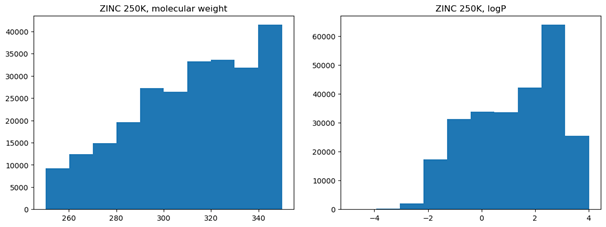
\includegraphics[width=0.75\linewidth]{zinc_descr.png}
    \caption{Enter Caption}
    \label{fig:zinc_descr}
\end{figure}

\subsubsection{ADME}

The ADME (absorption, distribution, metabolism, and excretion) dataset consists of 3521 diverse compounds which belong to 3028 distinct scaffolds. 2736 of these scaffolds contain only one molecule \cite{Fang.2023}. This should ensure a very high structural diversity (and make scaffold splitting rather unnecessary, see chapter methods). 
ADME processes ; for potential drug candidates a balanced ADME profile is an essential property \cite{Fang.2023}.
Six properties are given: include human liver microsomal (HLM) stability reported as intrinsic clearance (Clint, mL/min/kg), MDR1-MDCK efflux ratio (MDR1-MDCK ER), solubility at pH 6.8 (ug/mL), rat liver microsomal (RLM) stability reported as intrinsic clearance (Clint, mL/min/kg), human plasma protein binding (hPPB) percent unbound, and rat plasma protein binding (rPPB) percent unbound.

For example, in \cite{Fang.2023} it is noted that the addition of 2D RDKit descriptors to the molecular graph representation improved the performance. 


Unfortunately, for two of the six properties the number of molecules for which information is available is very small. For the other properties, especially for solubility, the values are highly skewed (fig. \ref{adme_value_distribution}.

\begin{figure}
    \centering
    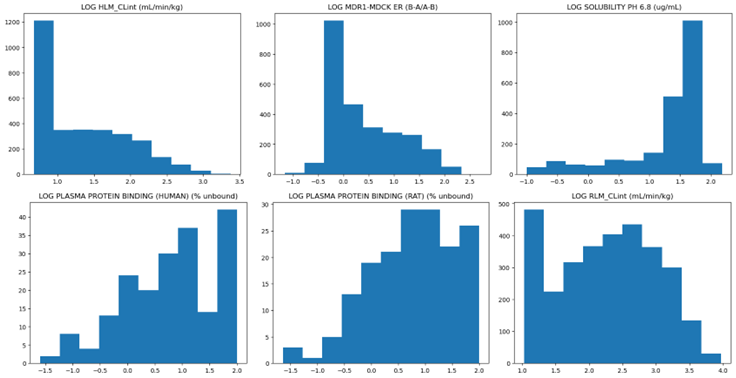
\includegraphics[width=1.1\linewidth]{adme_value_distribution.png}
    \caption{Distribution of the objective values in the ADME dataset}
    \label{fig:enter-label}
\end{figure}

\begin{table}[ht]
\centering
\begin{tabular}{|>{\raggedright\arraybackslash}p{5cm}|>{\raggedleft\arraybackslash}p{3cm}|}
\hline
\textbf{Total Molecules in dataset} & \textbf{3521} \\ \hline
\textbf{LOG HLM\_CLint (mL/min/kg)} & 3087 \\ \hline
\textbf{LOG MDR1-MDCK ER (B-A/A-B)} & 2642 \\ \hline
\textbf{LOG SOLUBILITY PH 6.8 (ug/mL)} & 2173 \\ \hline
\textbf{LOG PLASMA PROTEIN BINDING (HUMAN) (\% unbound)} & 194 \\ \hline
\textbf{LOG PLASMA PROTEIN BINDING (RAT) (\% unbound)} & 168 \\ \hline
\textbf{LOG RLM\_CLint (mL/min/kg)} & 3054 \\ \hline
\end{tabular}
\caption{Data table of different properties}
\end{table}

\begin{figure}
    \centering
    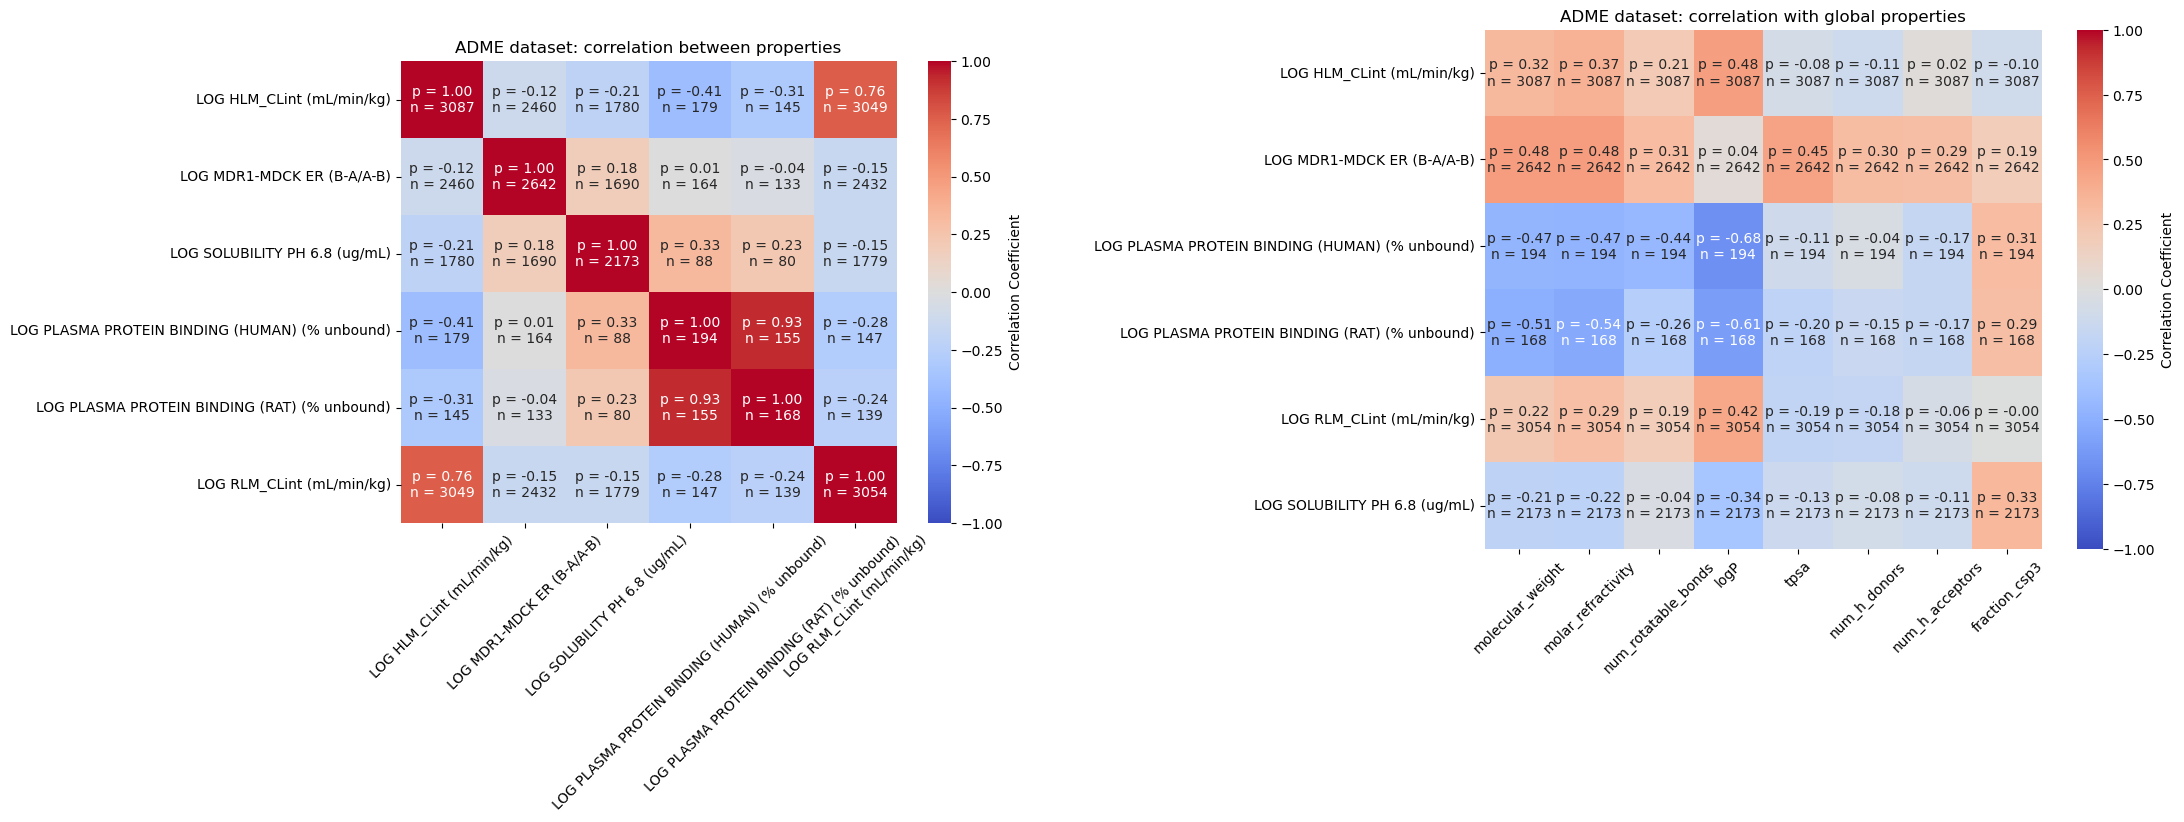
\includegraphics[width=1\linewidth]{adme_correlations.png}
    \caption{Enter Caption}
    \label{fig:enter-label}
\end{figure}

\subsubsection{Cancer data from NCBI}


\cite{He.2021} constructed a phenotypic screening data set comprising 13 breast cancer cell lines and one normal breast cell line.
The data was analyzed with with multiple GNNs, including a hybrid incorporating information from multiple fingerprint representations, but not the usual Morgan fingerprints.


In \cite{HernandezHernandez.2023} tested clustering approaches on data from the NCI-60 cancer cell line panel. was analyzed using graph representations.
\cite{Guo.2024} 
One of the examples investigated in this thesis is IGROV-1, a well-established cell line which acts as a model for drug-resistant ovarian carcinoma exhibiting low to moderate sensitivity to several common chemotherapeutic agents. \cite{Guo.2024} 



\subsubsection{LIT-PCBA}


The LIT-PCBA dataset aims to provide an unbiased dataset for machine learning and virtual screening. It consists of entries of bioactivity data from the PubChem BioAssay database (PCBA). 
It consists of 15 targets, 7844 active, and 407381 inactive compounds\cite{TranNguyen.2020}. The data set encompasses information from 149 dose-response PubChem bioassays. Properties like molecular weight are within a similar range for active and inactive compounds. False positives and assay artifacts were removed. All examples in LIT-PCBA are extremely imbalanced. For most proteins, only a few active compounds are given. This ratio mimics the setting of experimental screening.
Examples are the TP53 Cellular tumor antigen p53 inhibitor (602 actives, 10488 total) and the Estrogen receptor β antagonist (477 actives, 10486 total).

The corresponding ligand sets were unbiased by the asymmetric validation embedding (AVE) procedure. AVE systematically measures the pairwise distance in chemical space between molecules belonging to four sets of compounds. Since the unbiasing is based on ECFP4 fingerprints, one could assumed that it is ‘biased’ against the Morgan fingerprints.


\subsubsection{Activity data from ChEMBL}


A further activity dataset was proposed in \cite{CortesCiriano.2019}. It contains data from ChEMBL concerning the inhibition of diverse molecular compounds like the neurotransmitter dopamine, estrogen and the protein HERG which acts as a potassium ion channel. These molecular compounds are of great interest for drug discovery; e.g., inhibition of hERG is a side-effect of some drugs, leading to severe heart failure. 
In a similar vein, an opioid-related dataset from ChEMBL was assembled for benchmarking in \cite{Deng.2023}. It includes K-related targets like multi-drug resistance protein 1 (MDR1), cytochrome P450 2D6 (CYP2D6) and CYP3A4. Relevant PD-related targets include the μ-opioid receptor (MOR), δ-opioid receptor (DOR), and κ-opioid receptor (KOR).
In \cite{Deng.2023}, only classical fingerprint models and pretrained models like Grover and MolBERT were applied on these datasets. Fingerprints were never outperformed, but for smaller datasets they were much better than pretrained transformer models (for small data, MolBERT was worst by far). In the following, it will be investigated how graph representations perform on these datasets.

Two examples from the dataset are the neurotransmitter dopamine and hERG, the alpha subunit of a potassium ion channel essential for cardiac function, whose binding by drugs can lead to adverse side effects.

The selection investigated in this thesis was chosen in such a way that it provides a rather diverse subset, e.g. concerning data size as well as function, and allows, if possible, a direct comparison with the results in the publication it was firstly used. For example, IGROV-1 was presented as paradigmatic example in \cite{Zhang.2024}.

